\section{Study Area and Spatio-Temporal Framework}
\label{sec:study_area}

\subsection{Geographical Selection and Contrasting Climatic Biomes}
India exhibits extraordinary bioclimatic diversity, ranging from hyper-arid desert plateaus to tropical monsoon coastlines. To ensure that our compound modeling framework is not overfitted to a single environmental regime, we evaluate seven major metropolitan regions encompassing distinct K{\"o}ppen climate classifications, urban morphologies, and developmental trajectories (Table~\ref{tab:city_biomes}):

\begin{enumerate}
    \item \textbf{Bikaner (Hot Arid Desert, \textit{BWh}):} Located in the Thar Desert of Rajasthan, Bikaner experiences extreme thermal regimes ($>46^\circ\text{C}$ in summer, $<5^\circ\text{C}$ in winter), severe annual water deficits, and low vegetative cover amidst moving sand dunes.
    \item \textbf{Coimbatore (Semi-Arid Rainshadow, \textit{BSh}):} Situated in the rainshadow of the Western Ghats in Tamil Nadu, Coimbatore exhibits moderate inland temperatures, bimodal seasonal rainfall, and rapid textile-driven peri-urban industrialization.
    \item \textbf{Delhi National Capital Region (Subtropical Semi-Arid Monsoon, \textit{Cwa}):} Situated in the Indo-Gangetic Plain, Delhi represents one of the world's most populous megacities, suffering from extreme pre-monsoon heatwaves, heavy monsoon downpours, and severe post-monsoon winter atmospheric stagnation and smog inversions.
    \item \textbf{Hyderabad (Tropical Semi-Arid, \textit{BSh}):} Anchored on the Deccan Plateau of Telangana, Hyderabad features undulating granitic topography, moderate annual rainfall, and localized flash-flood vulnerability driven by rapid urban lake encroachment.
    \item \textbf{Indore (Tropical Savanna Plateau, \textit{Aw}):} Located on the Malwa Plateau of Madhya Pradesh, Indore serves as a central commercial hub with a balanced tropical savanna climate and historically documented high civic sanitation benchmarks.
    \item \textbf{Kolkata (Humid Deltaic Subtropical, \textit{Aw}):} Spanning the lower Gangetic Delta in West Bengal, Kolkata experiences intense maritime humidity, severe urban heat island (UHI) amplification, high building footprint density, and coastal cyclone/tidal flood susceptibility.
    \item \textbf{Mumbai Metropolitan Region (Tropical Coastal Monsoon, \textit{Am}):} Sited along the Konkan Coast of Maharashtra, Mumbai represents a linear coastal megacity subject to extreme southwest monsoon deluges, persistent marine humidity, and dense coastal slum concentrations.
\end{enumerate}

\begin{table}[t]
\centering
\small
\caption{Characteristics of the seven study metropolitan regions across contrasting Indian climatic biomes (2020--2022 panel, Uber H3 Resolution~8).}
\label{tab:city_biomes}
\begin{tabularx}{\textwidth}{@{}l X r r r l@{}}
\toprule
\textbf{City} & \textbf{K{\"o}ppen Biome} & \textbf{H3 Hexes} & \textbf{Area (km$^2$)} & \textbf{Panel Obs.} & \textbf{Centroid Coordinates} \\
\midrule
Bikaner & Hot arid desert (\textit{BWh}) & 959 & 707 & 34,524 & $28.02^\circ\text{N}, 73.32^\circ\text{E}$ \\
Coimbatore & Semi-arid rainshadow (\textit{BSh}) & 995 & 733 & 35,820 & $11.01^\circ\text{N}, 76.96^\circ\text{E}$ \\
Delhi & Subtropical semi-arid (\textit{Cwa}) & 3,398 & 2,504 & 122,328 & $28.61^\circ\text{N}, 77.20^\circ\text{E}$ \\
Hyderabad & Tropical semi-arid (\textit{BSh}) & 1,505 & 1,109 & 54,180 & $17.38^\circ\text{N}, 78.48^\circ\text{E}$ \\
Indore & Tropical savanna plateau (\textit{Aw}) & 731 & 539 & 26,316 & $22.72^\circ\text{N}, 75.86^\circ\text{E}$ \\
Kolkata & Humid deltaic subtropical (\textit{Aw}) & 992 & 731 & 35,712 & $22.57^\circ\text{N}, 88.36^\circ\text{E}$ \\
Mumbai & Tropical coastal monsoon (\textit{Am}) & 707 & 521 & 25,452 & $19.07^\circ\text{N}, 72.88^\circ\text{E}$ \\
\midrule
\textbf{Total} & \textbf{7 Contrasting Biomes} & \textbf{9,287} & \textbf{6,844} & \textbf{334,332} & \textbf{Pan-India Cohort} \\
\bottomrule
\end{tabularx}
\end{table}


\subsection{Discrete Global Grid System: Uber H3 Resolution 8}
Spatial analyses of urban risk have historically suffered from the Modifiable Areal Unit Problem (MAUP), where arbitrary administrative wards distort spatial gradients. To establish an objective, invariant geometric partition, we utilize the Uber H3 Discrete Global Grid System \citep{brodsky2018h3}. 

We adopt \textbf{H3 Resolution~8}, which partitions the Earth's surface into regular hexagonal cells with an average area of $0.7374\text{ km}^2$ and an inter-centroid spacing of approximately $0.92\text{ km}$. Hexagonal tessellations provide uniform topological adjacency (each cell shares equidistant boundaries with exactly six contiguous neighbors), isotropic spatial kernel convolution, and the elimination of orthogonal shear distortion inherent in Cartesian raster grids.

Across the seven metropolitan extents, a total of \textbf{9,287 discrete hexagonal cells} are delineated. Monitored across the 36-month observation period from January 2020 through December 2022, the balanced spatio-temporal panel yields exactly:
\begin{equation}
    N = 9,287 \text{ cells} \times 36 \text{ months} = 334,332 \text{ spatio-temporal observations}
\end{equation}
No missing hex-months exist within the panel, ensuring a strictly balanced longitudinal panel structure suitable for two-way fixed-effects and variance decomposition models.

\begin{figure*}[t]
    \centering
    \IfFileExists{figures/Figure1_study_area_7_cities.png}{%
        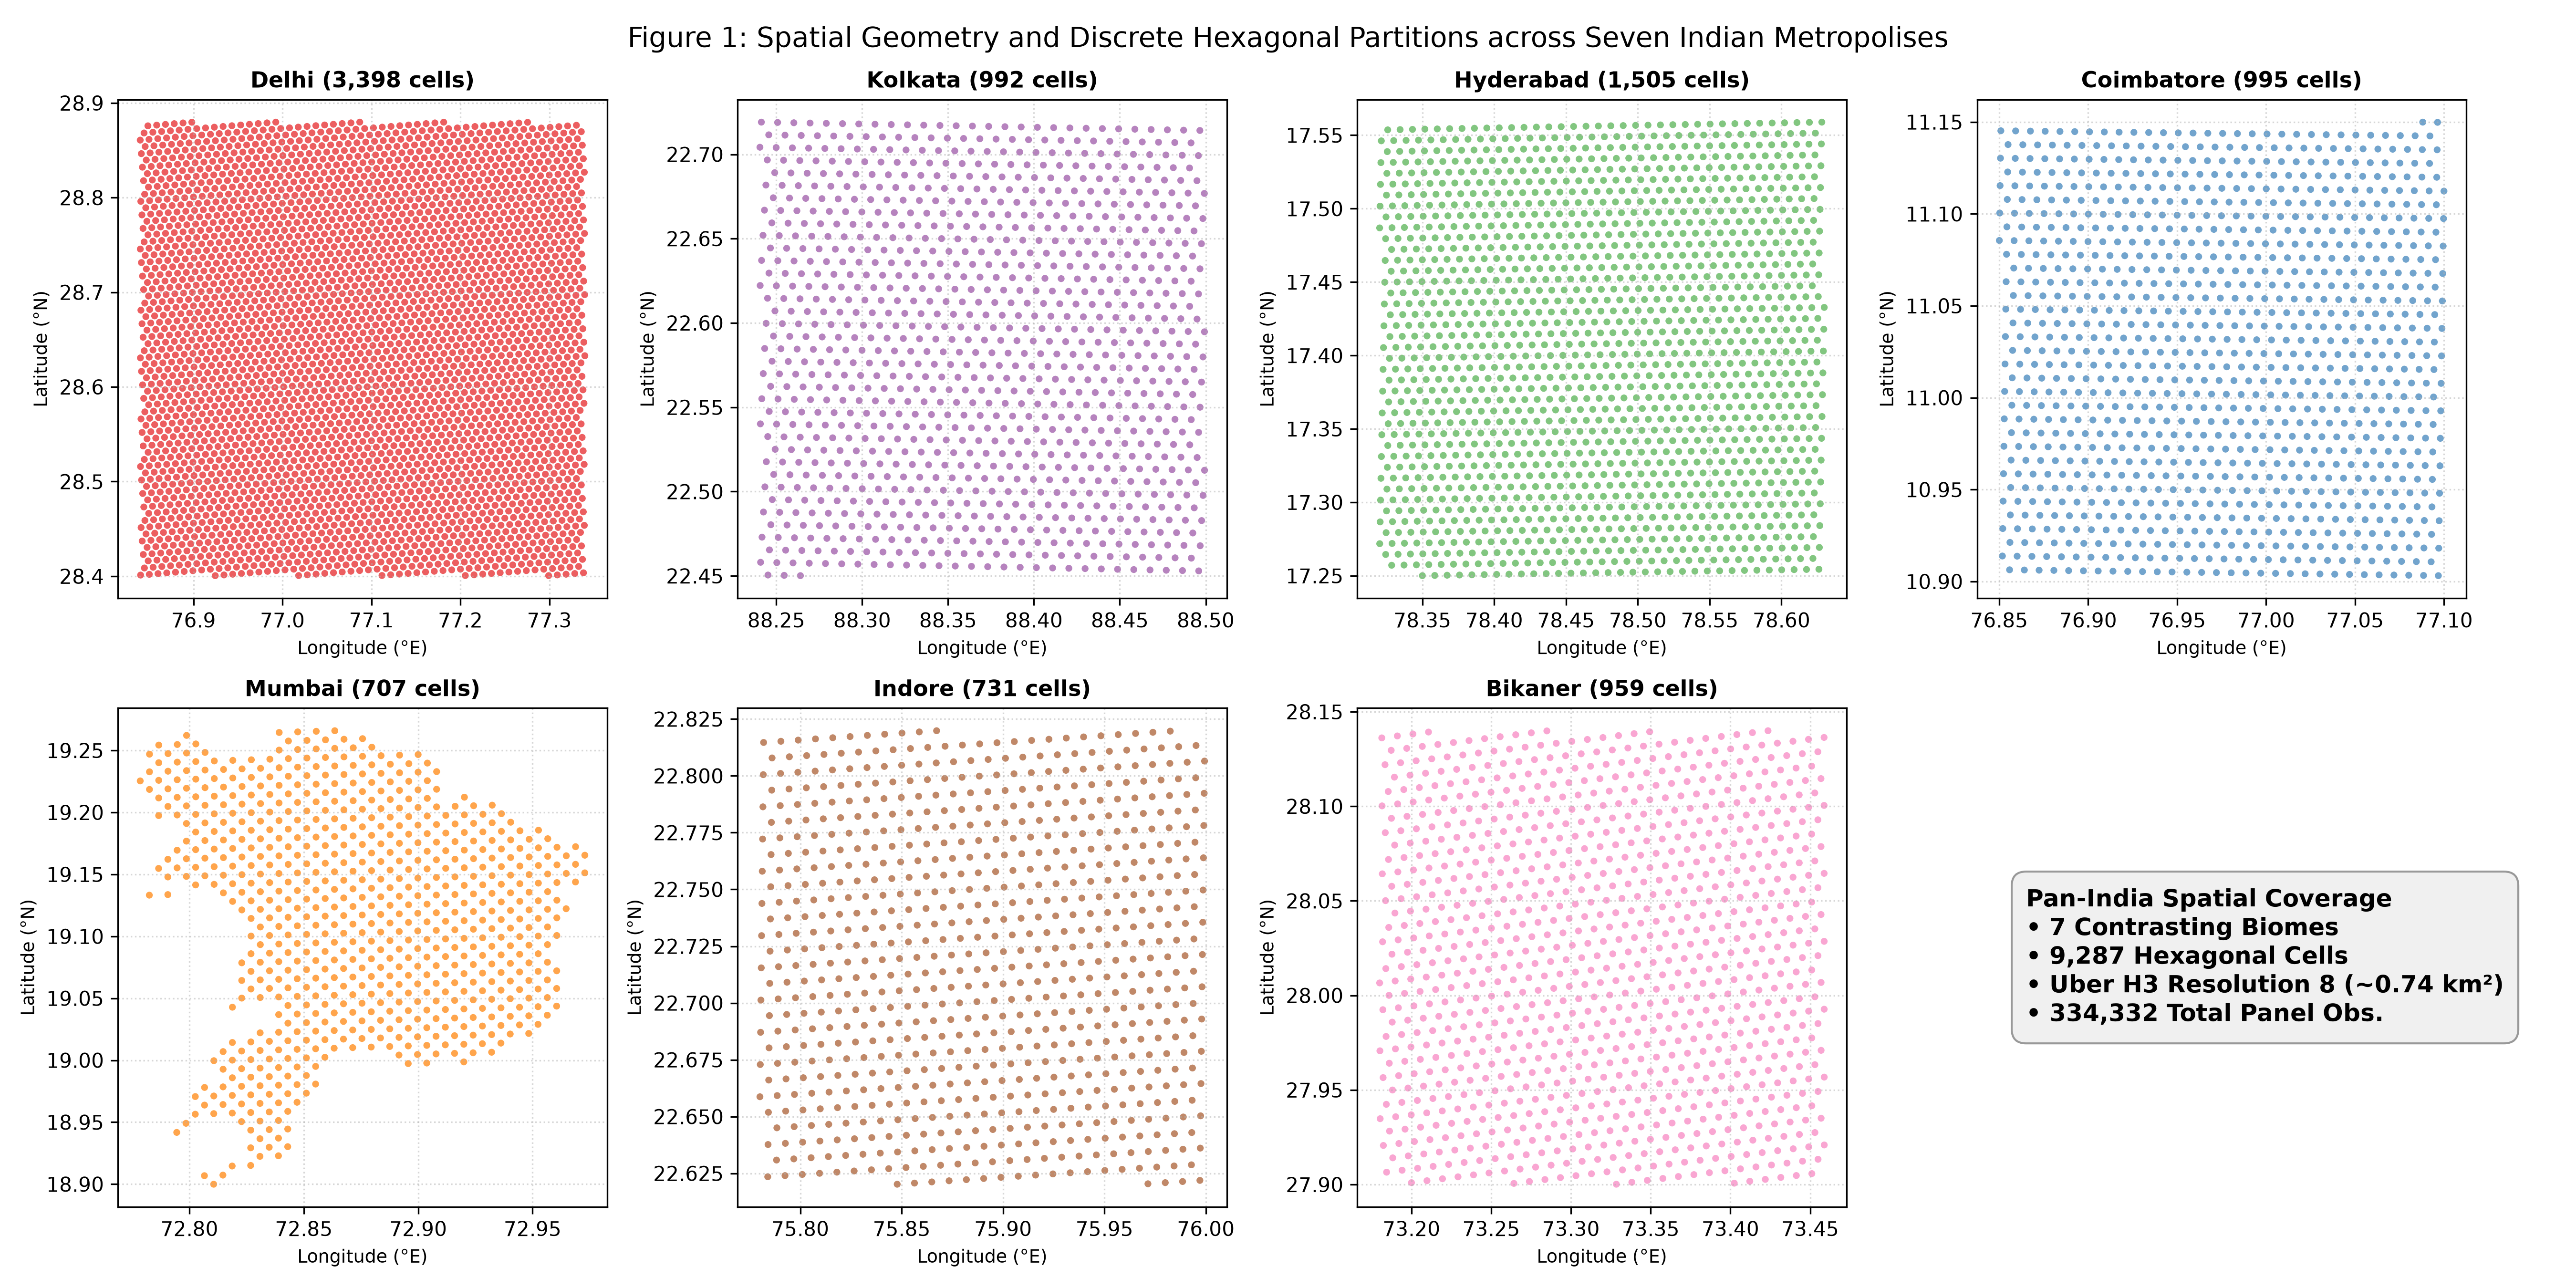
\includegraphics[width=\textwidth]{figures/Figure1_study_area_7_cities.png}%
    }{%
        \vspace{1em}
        \fbox{\parbox{0.95\textwidth}{\centering\small\textbf{[Figure 1: Spatial Geometry and Discrete Hexagonal Partitions Across Seven Indian Metropolises]}\\
        \textit{Generated via \texttt{colab\_analysis.py} from \texttt{final\_7\_cities.parquet}. Depicts all 9,287 Uber H3 Resolution 8 cells partitioned across the seven contrasting bioclimatic study regions.}}}%
        \vspace{1em}
    }
    \caption{Geographic distribution and discrete global grid tessellations (Uber H3 Resolution~8, $\sim 0.74\text{ km}^2$) for the seven study metropolises across India ($N = 334,332$ panel observations). Each cell provides uniform topological adjacency and isotropic spatial sampling, eliminating administrative boundary distortions.}
    \label{fig:study_area}
\end{figure*}
